\documentclass[a4paper,12pt]{article}
\usepackage[slovene]{babel}
\usepackage[utf8]{inputenc}
\usepackage[T1]{fontenc}
\usepackage{lmodern}
\usepackage{amsmath}
\usepackage{hyperref} 
\usepackage{graphicx} 
\usepackage{amsfonts}
\usepackage{eurosym}
\usepackage{stackengine}
\usepackage{fancyhdr}
\usepackage{amssymb}
\usepackage{graphicx}
\usepackage{amsbsy}
\usepackage{mathtools}
\usepackage{subcaption}
\usepackage{amsthm}
\usepackage{multirow}
\usepackage[output-decimal-marker={,}]{siunitx}
\theoremstyle{definition}
\newtheorem{definition}{Lema}
\begin{document}
\title{Robustni problem nahrbtnika}
\author{Eva Babnik in Jan Založnik}
\date{December, 2020}
\maketitle


\newpage
\tableofcontents
%\renewcommand{\listfigurename}{karkoli}
\listoffigures
\listoftables
\newpage
\section{Uvod}
\medskip
Namen tega poročila je, da predstaviva robustni problem nahrbtnika in kodo s katero sva ga rešila. Kodo bova sproti 
ustrezno komentirala ter dodala njeno časovno zahtevnost. Vključila bova tudi nekaj primerov in zraven dodala še časovne vrednosti, ki jih je program
potreboval za izračun rešitve. Program bova potem poskušala uporabiti na finančnem modelu. Podatke iz ameriške borze bova
uporabila na kodi za robustni problem in tako poskušala sestaviti optimalni portfelj. Prav tako bova tudi tu dodala primere in 
njihovo časovno zahtevnost.

\section{Povzetek}
\medskip
Poročilo se prične s kratko predstavitvijo navadnega oziroma klasičnega problema nahrbtnika in nato še z razlago 
robustnega problema nahrbtnika. Prav tako kot v klasičnem primeru problema nahrbtnika tudi pri robustnemu problemu iščemo 
množico predmetov, ki jih bomo položili v nahrbtnik in njihovo optimalno vrednost, vendar v tem primeru nimamo točnih podatkov o 
vseh težah predmetov. Za njihove teže vemo le, da so element določenega zaprtega intervala, ki torej ima zgornjo in spodnjo mejo.
Poleg intervalov tež predmetov pa še vemo maksimalno število elementov, ki lahko spremeni svojo težo, to število označimo z $\Gamma$.
\paragraph{}
Za sledeči problem sva s pomočjo dinamičnega programiranja napisala rekurzivne enačbe, na katerih bazira
najina koda v programskem jeziku \textit{python}. Napisala sva program, ki reši tako klasični problem nahrbtnika kot 
tudi robustni problem nahrbtnika in za rešitev vrne optimalni seznam predmetov, ki jih položimo v nahrbtnik in skupno 
optimalno vrednost le-teh. Sestavila pa sva tudi enostavnejši grafični prikaz, ki omogoča, da lahko problem reši tudi posameznik, 
ki nima nikakršnega predznanja v programiranju.
\paragraph{}
Nato sva kodo malo modificirala in jo uporabila na poenostavljenem finančnem modelu. 
Program prebere datoteko s podatki, ki zajemajo ceno delnice, najvišjo možno ceno delnice in letno stopnjo donosa, vrne pa 
optimalni portfelj, ki si ga lahko izberemo, če imamo za investicije na voljo  določeno vsoto denarja.




\newpage
\section{Problem nahrbtnika}
\medskip
Klasični problem nahrbtinka (angl. \textit{classical Knapsack Problem}) je računalniški problem, s katerim poskusimo zapolniti 
nahrbtnik z danimi predmeti, pri čem ima vsak svojo ceno in težo. Bodisi gre za dejansko polnjenje nahrbtnika, polnjenje 
nakupovalne vreče ali morda zlaganje predmetov v avto. V nadaljevanju poročila bova za klasični problem uporabljala kar kratico KP. 
Na voljo imamo množico $n$-tih predmetov, ki jo označimo z $N = \{1, \dots, n\}$ in nahrbtnik s kapaciteto $c$. Vsak predmet ima 
pozitivno vrednost $p_{j}$ in pozitivno utež $w_{j}$. Problem nahrbtnika nas sprašuje, katero podmnožico predmetov iz $N$ moramo 
položiti v nahrbtnik, da bo skupna vrednost le teh čim večja možna in da ne bo presegla nahrbtnikove kapacitete. 
Torej maksimiziramo skupno vrednost predmetov pri pogoju, da seštevek izbranih uteži ne presega nahrbtinkove zmogljivosti.
Problem lahko predstavimo kot celoštevilski linearni program (CLP):


\begin{equation}
    \tag*{}
     max \sum_{j \in N} p_{j}x_{j}
\end{equation}
\begin{equation}
    \tag*{}
    \sum_{j \in N} w_{j}x_{j} \leq c
\end{equation}
\begin{equation}
    \tag*{}
    x_{j} \in \{0,1\}, j \in N
\end{equation}

\medskip
\noindent Kjer $x_{j}$ zavzame vrednost 1, če $j$-ti predmet položimo v nahrbtnik,
 sicer zavzame vrednost 0. 

\section{Robustni problem nahrbtnika}
\medskip
Robustni problem nahrbtnika (angl. \textit{Robust Knapsack Problem}) v nadaljevanju 
RKP, je nekakšna nadgranja problema nahrbtnika. Dodaten problem se pojavi pri točnosti 
naših podatkov, in sicer pri utežeh $w_{j}$. Vsak predmet $j$ ima svojo nominalno težo 
$w_{j}$, ki pa je lahko netočna, ampak zanjo vemo, da se nahaja na intervalu 
[$w_{j} - \underline{w}_{j}$, $w_{j} + \overline{w}_{j}$]. Podan imamo tudi celošteviski parameter $\Gamma$,
ki označuje največje možno število predmetov z netočno izmerjeno težo. Pri iskanju 
rešitve problema moramo torej paziti, da bo seštevek vseh novih uteži še vedno manjši od
kapacitete nahrbtnika. Težav z rešitvijo seveda ne bomo imeli, če bodo vse dejanske uteži
nižje oziroma lažje od njene nominalne vrednosti, lahko pa se zgodi tudi najslabši možni 
izid, ko vse uteži zavzamejo zgornjo mejo intervala. Dopustno rešitev, kjer je
$J \subseteq N$ lahko formuliramo na naslednji način: 
\begin{equation}
    \tag*{}
    \sum_{j \in J}w_{j} + \sum_{j \in \hat{J}}\overline{w}_{j} \leq c,\quad \forall \hat{J} \subseteq J \; \text{in}\; |\hat{J}| \leq \Gamma 
\end{equation}
Zaradi lažje notacije v nadaljevanju definirajmo povečano težo kot $\hat{w}_j = w_j + \overline{w}_{j}$ za vsak $j$.
\section{Pristop z dinamičnim programiranjem}   %pobravano rumeno ker je č noter :/
\medskip
Naj bo $ \bar{z}(d, s, j) $ najvišji dobiček za dopustno rešitev s skupno težo $d$, kjer so upoštevani 
samo elementi iz množice $\{1, \dots,j\} \in N$ in samo $s$ izmed njih doseže zgornjo mejo $\hat{w}_j$. 
Naj bo $z(d, j)$ največji dobiček za dopustno rešitev s skupno težo $d$, kjer so upoštevani samo elementi 
iz množice $\{ 1,\dots,j \} \in N $ in naj jih le $\Gamma $ spremeni težo iz nominalne na zgornjo mejo $\hat{w}_j$. 
Torej velja $d = 0, 1, \dots, c$; $s = 0, 1, \dots, \Gamma$ in $ j = 0, 1, \dots, n$.
Ključna lastnost pravilnosti tega pristopa je predpostavka, da so predmeti razvrščeni po padajoči teži $\overline{w}_j$. 
To predpostavko nakazuje naslednja lema. Za podmnožico elementov
 $J \subseteq N$ z $j_\Gamma$ označimo indeks $\Gamma$-tega elementa v $J$, če
 je $|J| \geq \Gamma$, v nasprotnem primeru pa $j_\Gamma$ predstavlja indeks 
 zadnjega elementa v $J$. 
\begin{definition}\label{lema1}
Podmnožica $J \subseteq N$ je dopustna rešitev natanko tedaj ko velja:
\begin{equation}
    \tag*{}
        \sum_{j \in J|j \leq j_\Gamma} \hat{w}_j + \sum_{j \in J|j > j_\Gamma}w_j \leq c
\end{equation}
\end{definition}
\begin{proof}
    Največja rast vsote nominalnih tež vseh predmetov iz $J$, ki jo
    povzročijo predmeti, ki dosežejo svojo zgornjo težo, se zgodi zaradi 
    podmnožice stvari $\Gamma$, v kateri je $\overline{w}_j$ najvišji. Če je
    $J$ dopustna rešitev glede na to podmnožico, bo dopustna za katerokoli drugo
    podmnožico $J$.
\end{proof}
Problem lahko zapišemo z naslednjimi rekurzivnimi zvezami: 
\begin{equation}  
    \tag*{}
    \begin{matrix}
    \bar{z}(d, s, j) = max\{ \bar{z}(d, s, j - 1), \bar{z}(d - \hat{w}_j, s- 1, j - 1) + p_j\} \\
    \text{za} \; \; d = 0,\dots, c; \; s = 1,\dots, \Gamma \:\: \text{in} \:\:j = 1,\dots, n. \\ 
    \\
    z(d, j) = max\{z(d, j - 1), z (d - w_j, j - 1) + p_j\} \\
    \text{za} \; \; d = 0,\dots, c\;\;\text{in}\;\: j = \Gamma + 1,\dots, n.
    \end{matrix}
\end{equation} 

\noindent Začetna vrednost je $\bar{z}(d, s, 0) = -\infty$ za $d = 0, \dots,c$ in s = $0, \dots, \Gamma$. 
Nato nastavimo $\bar{z}(0, 0, 0) = 0$. Oba zapisa sta med seboj povezana z enakostjo $z(d, \Gamma) = 
\bar{z}(d, \Gamma, \Gamma\}$ za vsak $d$. Optimalno vrednost robustnega problema nahrbtnika dobimo kot:
\begin{equation}
\tag*{}
z^{*} = max \begin{cases}
max\{z(d, n) |\; d = 1, \dots, c \\
max\{\bar{z}(d, s, n) |\; d = 1, \dots, c; \;s = 1, \dots, \Gamma -1\}
\end{cases}
\end{equation}
\medskip
kjer porabimo tudi celotno kapaciteto nahrbtnika $c^{*} \leq c$.
\par
Algoritem dinamičnega programiranja je sestavljen iz dveh korakov. V prvem koraku dobimo optimalno 
rešitev, ki vsebuje največ $\Gamma$ elementov s povečano težo. V drugem koraku pa nato dobljeno 
rešitev lahko razširimo z dodatnimi elementi z nespremenjeno težo. Algoritem lahko razdelimo na dva 
koraka, ker razvrstitev predmetov po padajoči teži $\bar{w}_j$ zagotavlja, da so v vsaki rešitvi 
elementi z najmanjšimi indeksi (torej tisti, ki so bili v nahrbtnik položeni prej) tisti, ki bodo 
dosegli večjo težo.

\section{Opis kode}
V mapo \textit{python}, natančneje v \textit{koda\_RKP.py} na repozitoriju sva dodala kodo, napisano v \textit{pythonu}, ki je ustrezno komentirana pri vseh bolj zapletenih 
funkcijah, tukaj pa bova še podrobneje prikazala funkciji \textit{solve\_RKP} in \textit{rekurzija}, ki sta glavni komponenti
za izračun RKP. Kot je že bilo omenjeno, je zelo pomembno, da so predmeti razvrščeni po padajoči teži $\bar{w}_j$, zato je najlažje 
če napišemo dodatno funkcijo, ki sama razporedi podatke v pravilni vrstni red, da nam to ni potrebno delati ročno. 
\medskip
\subsection{Solve\_RKP}
\begin{figure}[h]
    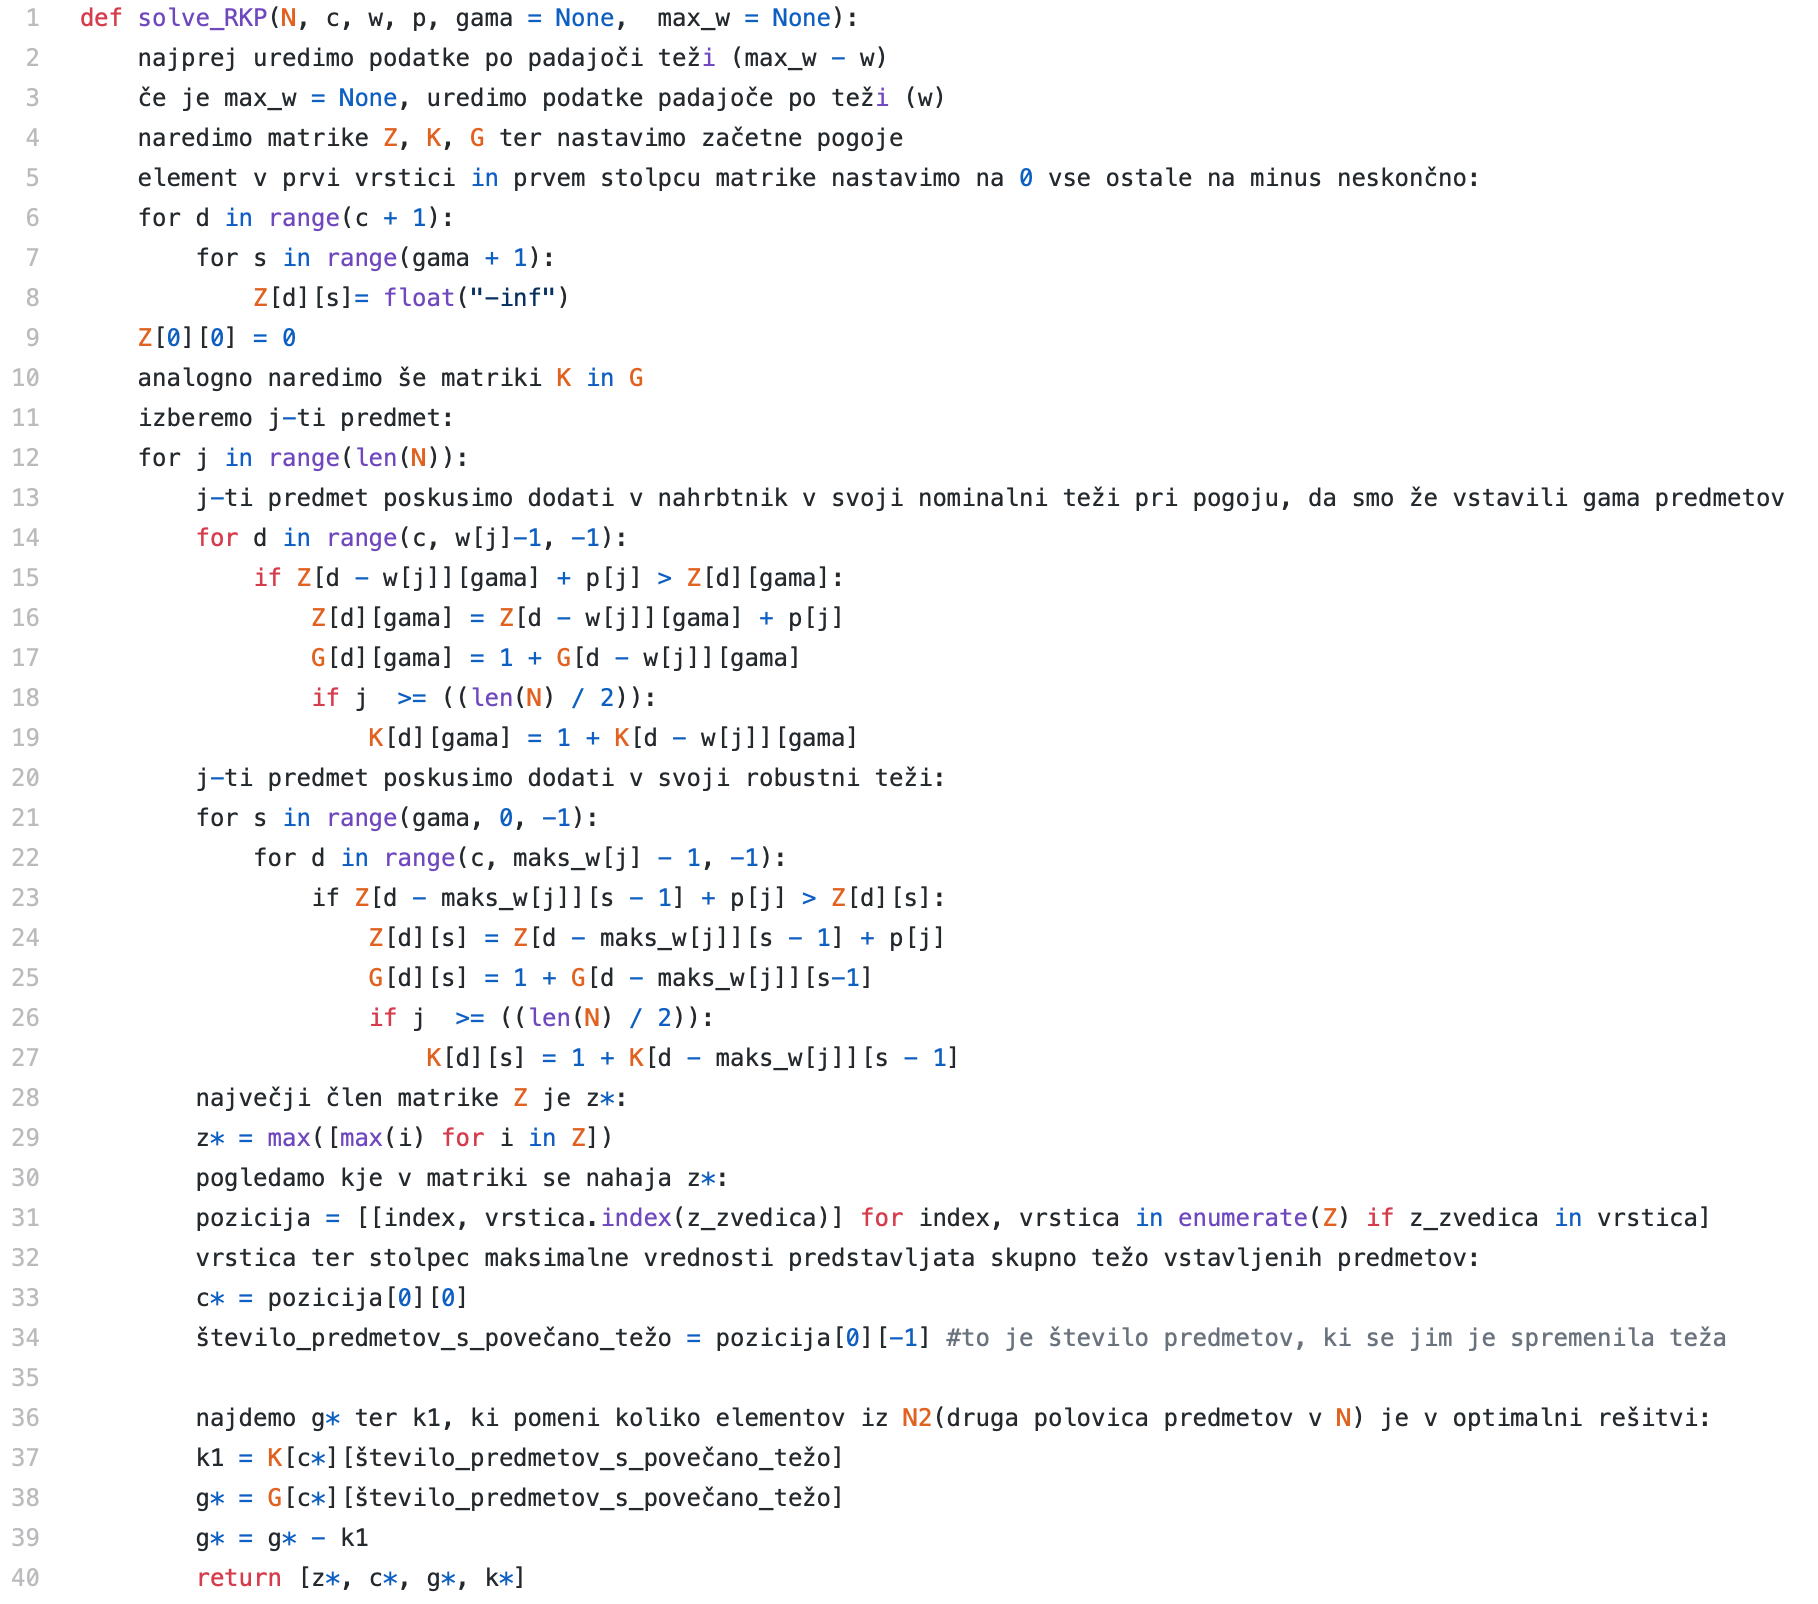
\includegraphics[width=13cm]{prava_RKP.png}
    \caption{Skica kode \textit{solve\_RKP}}
    \label{fig:koda1}    
\end{figure}

\paragraph{}
\noindent Funkcija \textit{solve\_RKP} sprejme štiri obvezne argumente: množico predmetov $N$ oblike
$\{1, \dots, n\}$, kjer je $n$ število predmetov; kapaciteto nahrbtnika $c$; teže predmetov $w$; vrednosti predmetov $p$ in dva neobvezna
argumenta $\Gamma$, ki označuje maksimalno število predmetov s spremenjeno težo ter $max\_w := \hat{w}$, ki prikazuje robustne teže predmetov. 
Vrne nam sledeče podatke: $z^{*}$ (optimalna vrednost predmetov, ki bodo v nahrbtniku), $c^{*}$ (optimalno težo predmetov v nahrbtniku), $g^{*}$ (število 
predmetov, ki jih damo v nahrbtnik) ter $k^{*}$ (število predmetov iz prve polovice množice $N$, ki jih dodamo v nahrbtnik). Vse te optimalne 
vrednosti potrebujemo kasneje v funkciji \textit{rekurzija}, da lahko dobimo seznam predmetov, ki jih bomo položili v nahrbtnik. V primeru ko 
ne podamo neobveznih argumentov $\Gamma$ in $max\_w$ nam funkcija \textit{solve\_RKP} vrne podobne optimalne vrednosti kot prej, le da tokrat 
reši KP.
\par

\subsubsection{Primer Solve\_RKP}

Recimo, da imamo 10 predmetov, ki jih želimo položiti v nahrbtnik s kapaciteto 20 kilogramov. Recimo, da so podatki za te predmete sledeči: 
$N = \{1, \dots, 10\}$, $c = 20$, $w = [4, 2, 6, 5, 2, 1, 7, 3, 5, 2]$, $p = [8, 5, 17, 10, 14, 4, 6, 8, 9, 25]$, $\Gamma = 4$, 
$max\_w = [5, 4, 6, 7, 4, 4, 7, 4, 5, 3]$, kjer so podatki $w$ in $max\_w$ predstavljeni v kilogramih, podatki $p$ pa v evrih. Če sedaj ta problem 
rešimo s funkcjo \textit{Solve\_RKP} dobimo naslednjo rešitev:

\begin{figure}[h]
    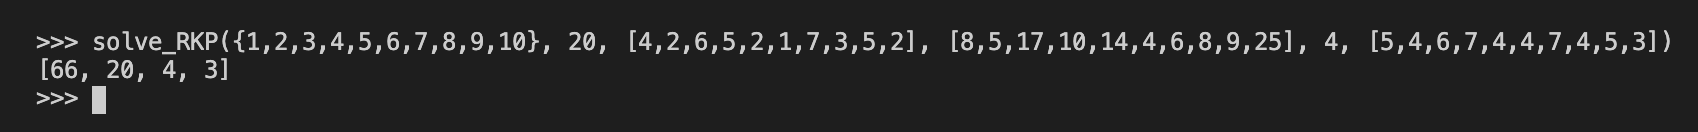
\includegraphics[width=14cm, height = 1.4cm]{primer1.png}
    \caption{Rešitev 1. primera}
    \label{fig:koda3}    
\end{figure}

\noindent Funkcija \textit{solve\_RKP} nam vrne seznam iz katerega razberemo, da je optimalna rešitev 66
 \euro, v nahrbtnik bomo položili $4$ predmete od tega $3$ predmete iz prve polovice množice predmetov $N$ ter da bomo nahrbtnik čisto napolnili.


\subsection{Rekurzija}
\medskip

\begin{figure}[h!]
    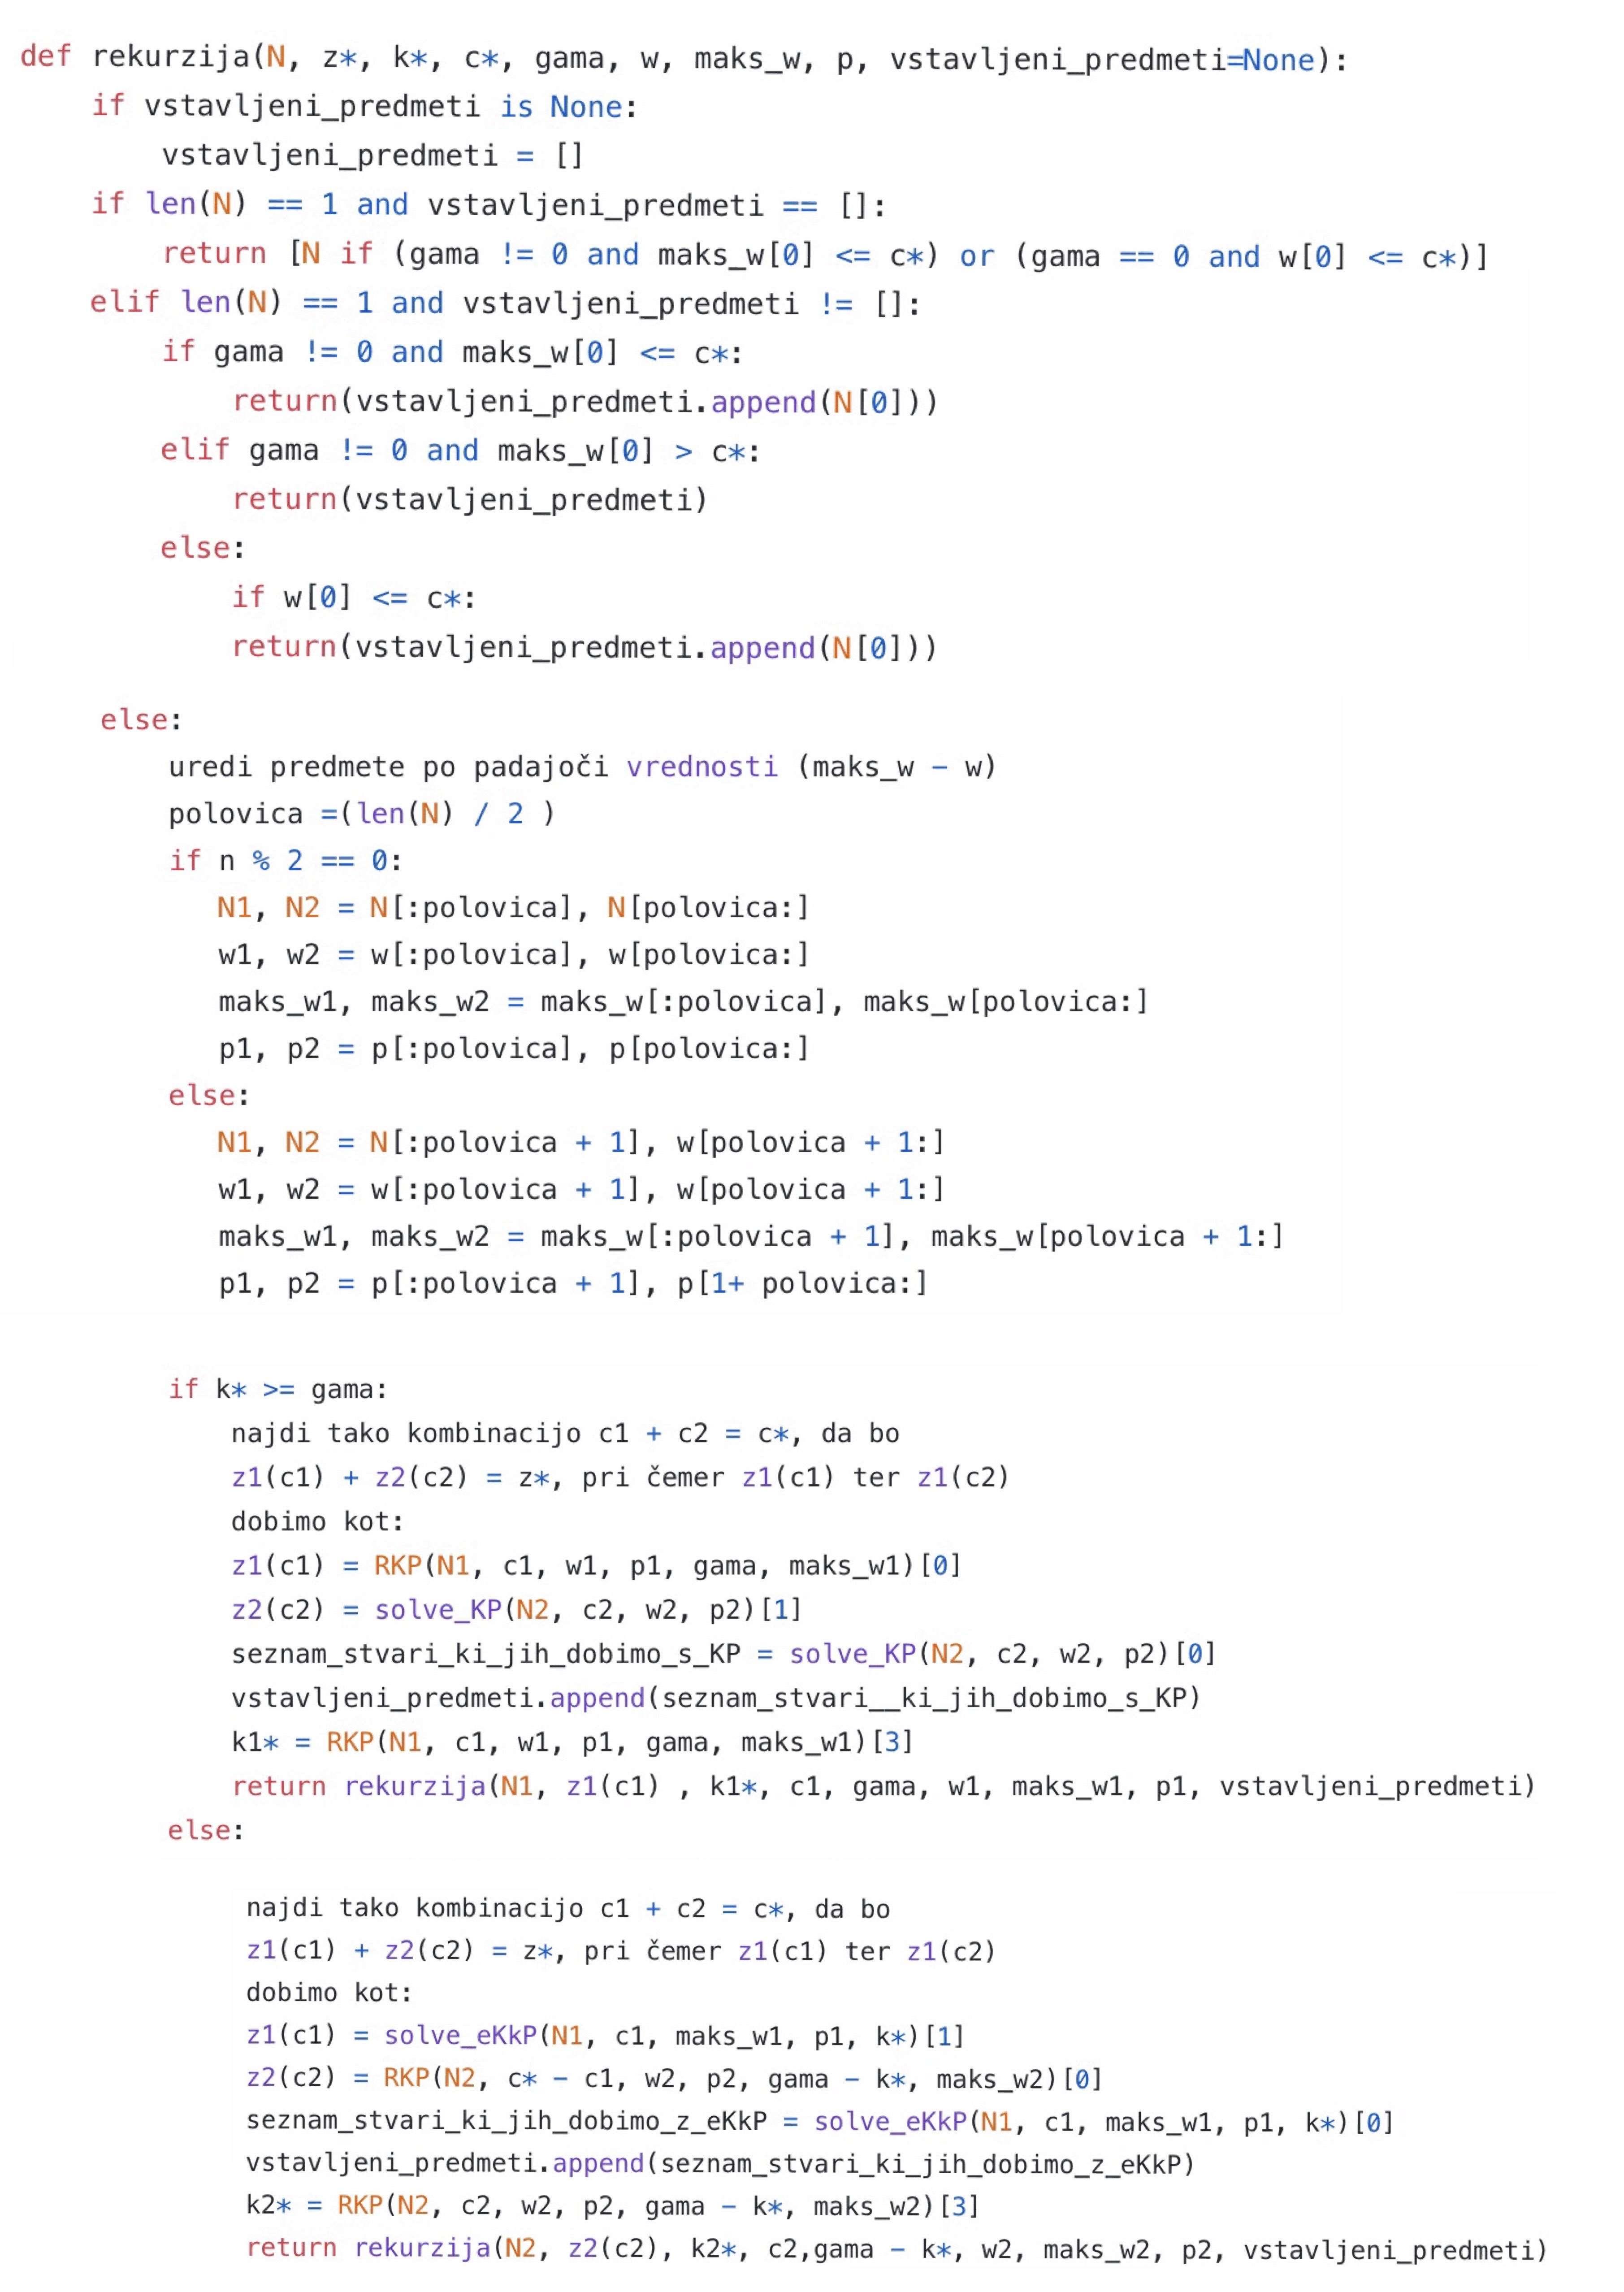
\includegraphics[width=13cm]{rekurzija.JPG}
    \caption{Skica kode \textit{rekurzija}}
    \label{fig:koda4}    
\end{figure}

Optimalni seznam stvari, ki jih vstavimo v nahrbtnik sva dobila s pomočjo funkcije $rekurzija$,
ki sprejme argumente $N, z^*, k^*, c^*,  \Gamma, w, \hat{w}, p$ in neobvezen argument 
$rešitev$,  pri čemer sva množico stvari $N$ razdelila na dva dela: $N = N_1 \cup N_2$ , za 
katera velja $N_1 = \{1, ..., n / 2\} $ in $N_2 = \{n / 2 + 1, ..., n\}$. Za primer ko je $n$ 
liho število, pa sva za elemente množice $N_1$ vzela prvih $\frac{n +1}{2} $ predmetov. Po izračunu
optimalne vrednosti s pomočjo funkcije $solve_RKP$ sva optimalni seznam stvari dobila rekurzivno za 
vsako množico stvari $N_i$, pri čemer sva si pomagala še z dvema funkcijama, pri katerih gre 
za različici problema nahrbtnika; s funkcijo \textit{Solve\_KP}, ki reši navadni problem
nahrbtnika, ki je opisan na začetku poročila in s funkcijo \textit{Solve\_eKkP}, ki reši 
problem nahrbtnika z omejenim številom predmetov, ki je podoben navadnemu problemu nahrbtnika, 
le da tu dodamo še omejitev:
\begin{equation}
\tag*{}   
\sum_{i=1}^{n}x_i = k
\end{equation} kjer $k$ pomeni dovoljeno število predmetov v nahrbtniku.
Najina delitev problema na dva dela temelji na naslednji lemi:
\begin{definition}
Če je $k^* \geq \Gamma$, potem je optimalna rešitev sestavljena iz rešitve za robustni problem 
nahrbtnika s parametrom $\Gamma$ za predmete iz množice $N_1$ in iz rešitve za navadni problem 
nahrbtnika za predmete iz množice $N_2$, pri čemer upoštevamo njihove nominalne teže. 
V primeru ko  je $k^* < \Gamma$, pa je optimalna rešitev sestavljena iz rešitve za
\textit{eKkP} s parametrom $k^*$ za predmete iz množice $N_1$ z njihovimi maksimalnimi 
težami in iz rešitve za robustni problem nahrbtnika s parametrom   $\Gamma - k^*$ za predmete 
iz množice $N_2$.
\end{definition}
\begin{proof}
    V \ref{lema1} je bilo povedano, da v vsaki dopustni rešitvi
    in torej tudi v optimalni rešitvi $\Gamma$ stvari z najnižjimi
    indeksi do $j_\Gamma$, so to tisti indeksi, ki h kapaciteti prispevajo
    njihovo najvišjo težo, vsi ostali predmeti z višjimi indeksi
    pa v nahrbtinku zavzemajo svojo nominalno težo. 
    \par
    Če je $k^* \geq \Gamma$, potem je $j_\Gamma \in N_1$ in vsi predmeti
    iz optimalne rešitve, ki pripadajo $N_2$, h kapaciteti prispevajo
    svojo nominalno težo.
    Če je $k^* < \Gamma$, potem je $j_\Gamma \in N_2$ in $k^*$
    predmetov v optimalni rešitvi pripada mmnožici $N_1$ 
    ter h kapaciteti prispeva najvišjo težo. Ostalih največ
    $\Gamma - k^*$ predmetov, ki se jim poveča teža, pa se nahaja
    v množici $N_2$.
\end{proof}
\subsubsection{Primer \textit{rekurzije}}

Recimo, da imamo iste podatke kot v primeru 6.1.1 in vrednosti $z^{*}$, $c^{*}$ ter $k^{*}$, ki jih dobimo 
iz rešitve \textit{solve\_RKP}. Podatke vstavimo v funkcijo \textit{rekurzija} in dobimo seznam predmetov, 
ki ji položimo v nahrbtnik: 

\begin{figure}[h]
    
\includegraphics[width=14cm, height = 1cm]{primer_rekurzija.png}
    \caption{Rešitev \textit{rekurzije}}
    \label{fig:koda6}    
\end{figure}

\section{Grafični vmesnik}

V mapi \textit{python}, natančneje v \textit{koda\_RKP} sva s pomočjo \textit{pythonove} knjižnice \textit{tkinter}
naredila aplikacijo z grafičnim vmesnikom. Ta vas najprej vpraša, kakšen tip problema imate, torej ali 
je to KP ali RKP in vam nato izbrani problem na kratko predstavi in vam pove, kako pravilno vnesti podatke 
na naslednji strani.

\begin{figure}[h!]
    \centering
    \begin{subfigure}[b]{0.8\linewidth}
      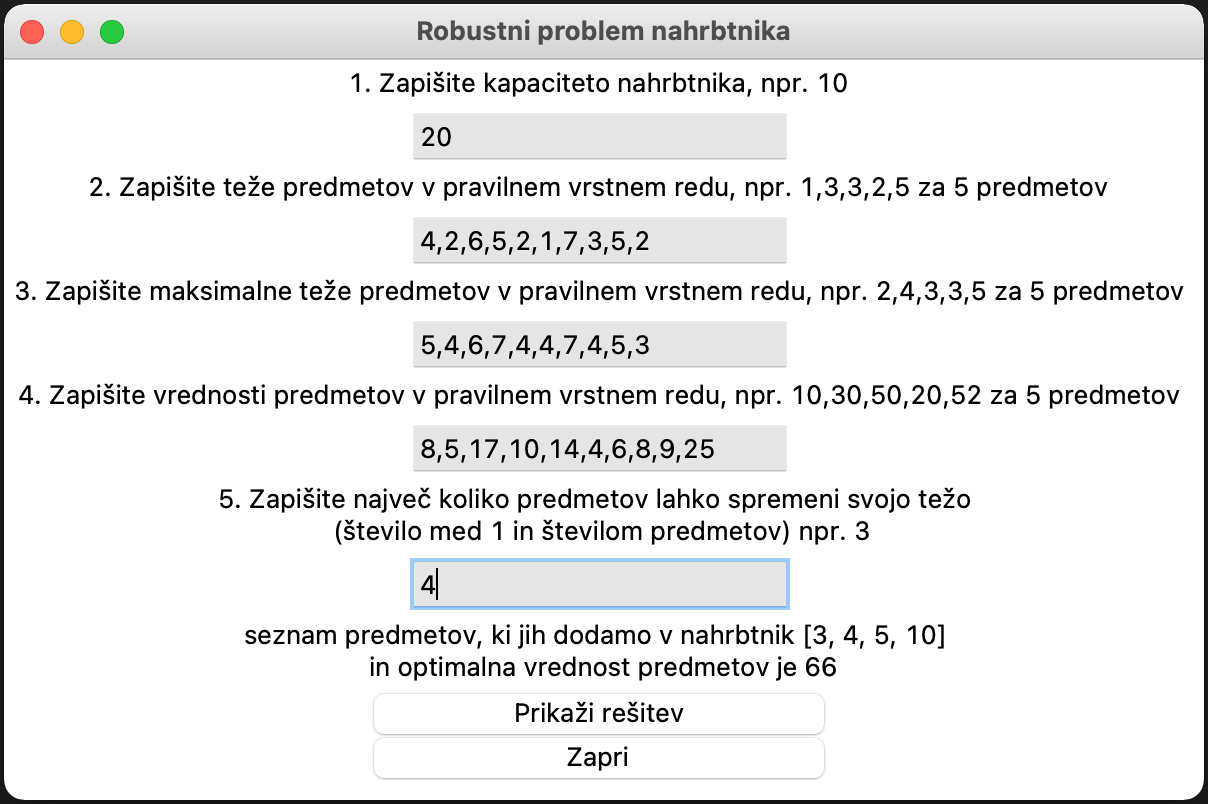
\includegraphics[width=\linewidth]{graficni_prikaz_RKP.png}
      \caption{Robustni problem nahrbtinka}
      \smallskip
    \end{subfigure}
    \begin{subfigure}[b]{0.8\linewidth}
      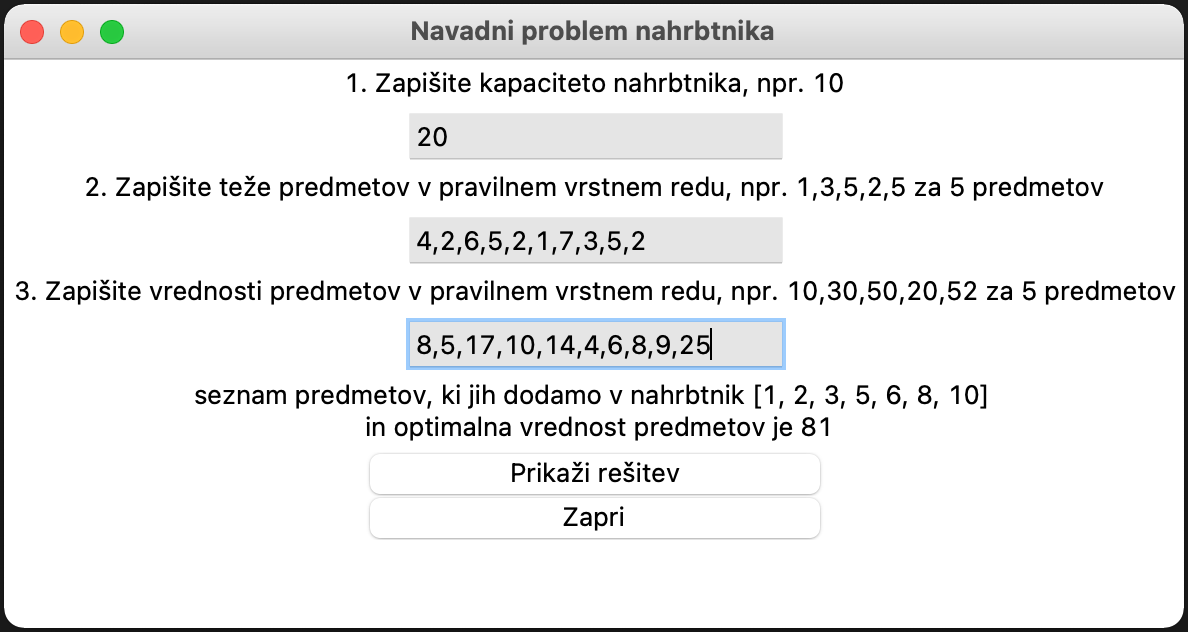
\includegraphics[width=\linewidth]{graficni_prikaz_KP.png}
      \caption{Navadni problem nahrbtinka}
    \end{subfigure}
    \caption{Primerjava istega primera v robustni in klasični obliki}
    \label{fig:koda2}
  \end{figure}

\noindent Če zopet uporabimo primer iz 6.1.1, nam bo aplikacija izpisala seznam predmetov, ki jih 
postavimo v nahrbtnik in optimalno vrednost predmetov, kot je razvidno iz slike \ref{fig:koda2}.a$)$. Če vstavimo 
iste podatke še v okno navadni problem nahrbtnika s to razliko, da je $\Gamma = 0$ dobimo optimalno vrednost 81 in 
seznam predmetov, ki jih položimo v nahrbtnik.

\section{Časovna zahtevnost in generirani podatki}
\medskip
Pogledali si bomo časovni zahtevnosti zgoraj opisanih funkcij, torej \textit{solve\_RKP}
in \textit{rekurzija}. 
Pri oceni časovne zahtevnosti funkcije \textit{solve\_RKP} 
si najprej poglejmo matrike $Z$, $K$, $G$. Ker se nahajajo v enakih 
zankah, je dovolj, da si pogledamo, kaj se med izvajanjem algoritma
dogaja z matriko $Z$, kjer gremo v zunanji zanki skozi vse elemente $j = 1, ...,n$.
Za vsak $j$ upoštevamo vse $s \leq \Gamma$, v notranji zanki pa gremo še
skozi vse možne kapacitete nahrbtinka $d = 0, ..., c$. Tako dobimo časovno zahtevnost
$\mathcal{O}(\Gamma n c)$.
Ko pokličemo funckijo \textit{rekurzija} ta v primeru,
ko je $k^* \geq \Gamma$ največ 
časa porabi pri klicanju funkcije \textit{solve\_RKP($c^*, \Gamma, N_1$)},
ki porabi $\mathcal{O}(\Gamma \frac{n}{2} c^*)$ časa in pri klicanju funkcije \textit{solve\_KP} s predmeti iz množice 
$N_2$, ki porabi $\mathcal{O}(\frac{n}{2} c^*)$ časa. V primeru,
 ko je $k^* < \Gamma$ pa funkcija največ časa porabi ko pokliče funkcijo \textit{solve\_EkKP} v času $\mathcal{O}(\Gamma \frac{n}{2} c^*)$
 in funckijo \textit{solve\_RKP} v času $\mathcal{O}(\Gamma \frac{n}{2} c^*)$. Časovna zahtevnost funkcije \textit{rekurzija}
 znaša torej $\mathcal{O}(\Gamma n c)$.
 \par
 V tabeli $($\ref{tab:tab1}$)$ je prikazana časovna zahtevnost algoritma v odvisnosti od $\Gamma$, $c$ in $n$, čas pa je merjen v sekundah.
 Vse meritve sva opravila s prenosnim računalnikom MacBook (early 2016) s procesorjem 1,2 GHz Dual-Core Intel Core m5 in 8GB spomina.
  Meritve sva izvedla na naključno generiranih podatkih, dobljenih s funkcijo \textit{naredi\_podatke}.
 Podatki se nahajajo v mapi \textit{podatki\_za\_merjenje\_časa}.
 
     
 
 \begin{table}[h]
    \centering
    \begin{tabular}{c|c|c|c|c|}
    \cline{3-5}
    \multicolumn{2}{c|}{}                                     & $c$ = 50  & $c$ = 100  & $c$ = 200  \\ \hline
    \multicolumn{1}{|c|}{\multirow{3}{*}{$n$ = 500}}  & $\Gamma$ = 1 & 0.9400  & 2.1294   & 7.4316   \\ \cline{2-5} 
    \multicolumn{1}{|c|}{}                          & $\Gamma$ = 10 & 2.1714  & 9.5391   & 36.5587  \\ \cline{2-5} 
    \multicolumn{1}{|c|}{}                          & $\Gamma$ = 50 & 7.4621  & 25.7643  & 97.5244  \\ \hline
    \multicolumn{1}{|c|}{\multirow{3}{*}{$n$ = 1000}} & $\Gamma$ = 1  & 1.4711  & 7.2800   & 16.7107  \\ \cline{2-5} 
    \multicolumn{1}{|c|}{}                          & $\Gamma$ = 10 & 6.2347  & 23.3414  & 77.9351  \\ \cline{2-5} 
    \multicolumn{1}{|c|}{}                          & $\Gamma$ = 50 & 11.1123 & 59.1479  & 302.4103 \\ \hline
    \multicolumn{1}{|c|}{\multirow{3}{*}{$n$ = 2000}} & $\Gamma$ = 1  & 4.3077  & 9.7543   & 37.6998  \\ \cline{2-5} 
    \multicolumn{1}{|c|}{}                          & $\Gamma$ = 10 & 14.2596 & 52.3112  & 195.0519 \\ \cline{2-5} 
    \multicolumn{1}{|c|}{}                          & $\Gamma$ = 50 & 26.1064 & 106.8547 & 700.8570 \\ \hline
    \end{tabular}
    \caption{\label{tab:tab1}Časovna zahtevnost algortima v odvisnosti od $n$, $\Gamma$ in $c$.}
\end{table}
\par
S pomočjo funkcije \textit{naredi\_podatke} sva zgenerirala nekaj naključnih podatkov, ki se nahajajo
v mapi \textit{generirani\_podatki}. Ime datoteke je sestavljeno kot \textit{podatki\_število\_predmetov\_c\_}$\Gamma$.txt.
Seznami stvari, ki jih vstavimo v nahrbtnik, se nahajajo v mapi \textit{resitve\_generiranih\_podatkov}.
\section{Optimizacija portfeljev s pomočjo RKP}
\medskip
Kodo za robustni problem nahrbtinka sva nato uporabila na poenostavljenem finančnem modelu,
kjer naju je zanimalo iz katerih delnic sestaviti optimalni portelj, pri čemer so cene delnic
negotove. 
\par
Recimo, da imamo M podjetij pri čemer imamo za vsako delnico podjetja $j$ na voljo nominalno ceno $P_j$,
interval [$P_j$ - $\underline{P}_{j}$, $P_j$ + $\overline{P}_{j}$], na katerem se cena delnice $p_j$  
nahaja in pričakovani donos delnice $R_j$. Zanima 
nas koliko delnic posameznega podjetja $j$ kupiti, da bo pričakovani dobiček čim višji in da ob tem nakupu
ne bomo presegli količine denarja $B$, namenjenega investiranju. Ob tem pa je potrebno tudi upoštevati,
da največ $\Gamma$ delnic podjetij spremeni svojo vrednost iz nominalne na maksimalno. Opisani primer lahko
formuliramo na naslednji način:
\begin{equation}
\tag*{}
     max \sum_{j \in M} P_{j}(1 + R_{j})N_{j}x_{j}
\end{equation}
\begin{equation}
\tag*{}
    \sum_{j \in M}P_{j}N_{j}x_{j} + \sum_{j \in \hat{M}}\overline{P}_{j}N_{j}x_{j} \leq B,\quad \forall \hat{M} \subseteq M \; \text{in}\; |\hat{M}| \leq \Gamma    
\end{equation}
\begin{equation}
\tag*{}
    p_{j} \in [P_{j} - \underline{P}_{j}, P_{j} + \overline{P}_{j}]
\end{equation}
\begin{equation}
\tag*{}
    x_{j} \in \{0,1\}, j \in M
\end{equation}
\begin{equation}
    \tag*{}
    N_j \in \{0, ..., \frac{B}{(P_j + \overline{P}_{j})} \}, j \in M
\end{equation}
Zaradi lažje notacije v nadaljevanju označimo $\hat{P}_j = P_j + \overline{P}_j$.
Da bi dobila rešitev tega modela sva kodi dodala
funkcije \textit{preberi\_podatke\_za\_delnice},
\textit{resitev\_za\_delnice} in \textit{doloci\_gamo}. Prva funkcija prebere
datoteko, v kateri so za vsako delnico podatki o imenu,
nominalni ceni, maksimalni ceni ter pričakovanem donosu.
Funkcija nato za vsako delnico izračuna največ koliko enakih
delnic po njihovi maksimalni ceni ob danem proračunu $B$ lahko kupimo in temu prilagodi sezname $P$,
$\hat{P}$ in $r$. Recimo, da je naš proračun enak $10$ in maksimalna cena delnice $i$ enaka
$5$, bomo torej delnico $i$ šteli dvakrat, prav tako pa bomo v zgoraj omenjenih seznamih
podvojili tudi njene vrednosti. Funkcija \textit{resitev\_za\_delnice} pa pokliče funkcijo \textit{rekurzija}
in nato poišče katere delnice pripadajo dobljeni optimalni rešitvi.
\par
$\Gamma$ tu ni podana skupaj s podatki, ampak jo iz podatkov izračunamo s pomočjo funckije \textit{doloci\_gamo}.
V tem modelu je $\Gamma$ namreč slučajna spremenljivka in jo lahko ob nekaterih predpostavkah (ki 
sicer v realnosti ne držijo popolnoma) dobimo verjetnostno, pri čemer sva predpostavila, da je $\Gamma$
binomsko porazdeljena. Najina ideja je bila torej ugotoviti, kdaj bo trenutna cena delnice $P_j$ narasla na 
$\hat{P}_j$. Sklepala sva, da večji pričakovani donos $R_j$ pomeni večjo verjetnost, da
bo cena delnice v danem trenutku narasla na $\hat{P}_j$, zato sva izračunala povprečen $R_j$, ki
sva ga označila z $\overline{R}$. 
Predpostavila sva, da je $\overline{R}$ kar enak verjetnosti $q$, ki predstavlja verjetnost,
da bo vrednost opazovanih delnic narasla. Nato sva s pomočjo funkcije $random.binomial(stevilo\_delnic, q)$ 
simulirala vrednosti slučajne spremenljivke $\Gamma$.
\par
Zaradi lažje preglednosti sva poosodobljeno kodo za finančni RKP model dala v datoteko
\textit{koda\_financni\_model\_RKP}, ki se nahaja v mapi \textit{python}. 
Za rešitev finančnega RKP modela potrebujemo dva argumenta; datoteko tipa \textit{.txt} (v kateri
so po vrsti v stolpcih napisani podatki: simbol podjetja, ime podjetja, nominalna cena delnice, 
najvišja cena delnice in pričakovani donos) ter znesek denarja, ki ga nameravamo nameniti investiranju.
Optimalni portelj dobimo tako, da pokličemo funkcijo \textit{resitev\_za\_delnice}(datoteka, budget)
\subsection{Uporaba RKP na delnicah $S\&P$ $500$}
Z zgoraj opisanim finančnim RKP modelom sva nato izračunala optimalni portfelj na podlagi 
o cenah in donosih delnic \textit{S}\&\textit{P 500}, kjer gre za 500 največjih in najbolj likvidnih
ameriških podjetij.  Najini 
podatki so vsebovali nominalno in najvišjo ceno ter pričakovani letni donos za delnice posameznih podjetij.
Iskala sva maksimalni donos portfelja glede na različne proračune $B$.
Ob tem je potrebno poudariti, da se zavedava, da dobljene rešitve niso najbolj optimalne, saj
ostalih dejavnikov, ki močno vplivajo na sestavo optimalnega portfelja (kot je npr. tveganje), 
sploh nisva upoštevala. V rezultatu dobimo zelo nerazpršen portfelj,
kar ni idealno, saj ravno z diverzifikacijo zmanjšujemo tveganje. 
\par
Optimalne portfelje za delnice \textit{S}\&\textit{P 500} sva izračunala za proračune $B = 50$, $B = 100$, $B = 500$,
$B = 1000$ in $B = 2000$. V tabeli $($\ref{tab:tab2}$)$ je prikazana časovna zahtevnost za posamezne 
primere v sekundah ter sestava optimalnega portfelja, pri čemer so imena podjetji zapisana z njihovimi
kraticami. 
\begin{table}[h]
    \resizebox{\textwidth}{!}{
    \begin{tabular}{c|c|c|c|c|c|}
    \cline{2-6}
                                                                                                  & B = 50                                                              & B = 100                                                                    & B = 500                                                                     & B = 1000                                                            & B = 2000                                                         \\ \hline
    \multicolumn{1}{|c|}{Čas}                                                                     & 3.9939                                                              & 8.0711                                                                     & 259.5398                                                                    & 931.2960                                                            & 5063.1349                                                        \\ \hline
    \multicolumn{1}{|c|}{\begin{tabular}[c]{@{}c@{}}Sestava optimalnega\\ portfelja\end{tabular}} & \begin{tabular}[c]{@{}c@{}}Carr: 1, Amcr: 1 \end{tabular} & \begin{tabular}[c]{@{}c@{}}Carr: 2, Xyl: 1,\\ Hwm: 1 \end{tabular} & \begin{tabular}[c]{@{}c@{}}Lb: 7, Etsy: 1\\ TPR: 1 \end{tabular} & \begin{tabular}[c]{@{}c@{}}Etsy: 5, Carr: 4,\\ Vtrs: 1\end{tabular} & \begin{tabular}[c]{@{}c@{}}Wts: 7, Wrk: 1,\\ Xyl: 1\end{tabular} \\ \hline
    \multicolumn{1}{|c|}{Dobiček}                                                                 & 75                                                                 & 173                                                                        & 766                                                                        & 3246                                                                & 3477                                                             \\ \hline
    \end{tabular}}
    \caption{\label{tab:tab2} Časovna zahtevnost finančnega RKP modela in dobljeni rezultati}
    
    \end{table}




\newpage
\section{Viri in literatura}

\begin{thebibliography}{9}

    \bibitem{RNP} 
    Michele Monaci, Ulrich Pferschy, Paolo Serafini 
    \\\texttt{https://www.sciencedirect.com/science/article/pii/S0305054813001342}

     \bibitem{podatki}
     Barchart. 
     \\\texttt{https://www.barchart.com/stocks/indices/sp/sp500}

     \bibitem{letni_donosi}
     Slickcharts.
     \\\texttt{https://www.slickcharts.com/sp500/performance}
\end{thebibliography}


\end{document}
